\documentclass[main.tex]{subfiles}

\begin{document}
\chapter{Parallelization of phonon calculations}\label{ch:optimization_ph}

The \texttt{PHonon} package enables calculations of phonon frequencies and eigenmodes.
This chapter examines the best ways to run \texttt{PHonon} calculations.
The benchmarks are averaged over 10 runs.

\section{Optimal parallelization parameters for phonon calculations}

As discussed in sec. \ref{sub:qe_parallelization}, the \texttt{PHonon} package offers the same three parallelization levels as the \texttt{PWscf} package, namely plane wave, k point and linear algebra parallelization.
Furthermore parallelization on q points (so called image parallelization) can be used.

\subsection{k point parallelization}

In a first step, the same k point parallelization benchmark as in sec. \ref{sub:scf_scaling_k_point} is run. This is depicted in fig. \ref{fig:scaling_ph_nk_si}.

\begin{figure}[htb!]
    \centering
    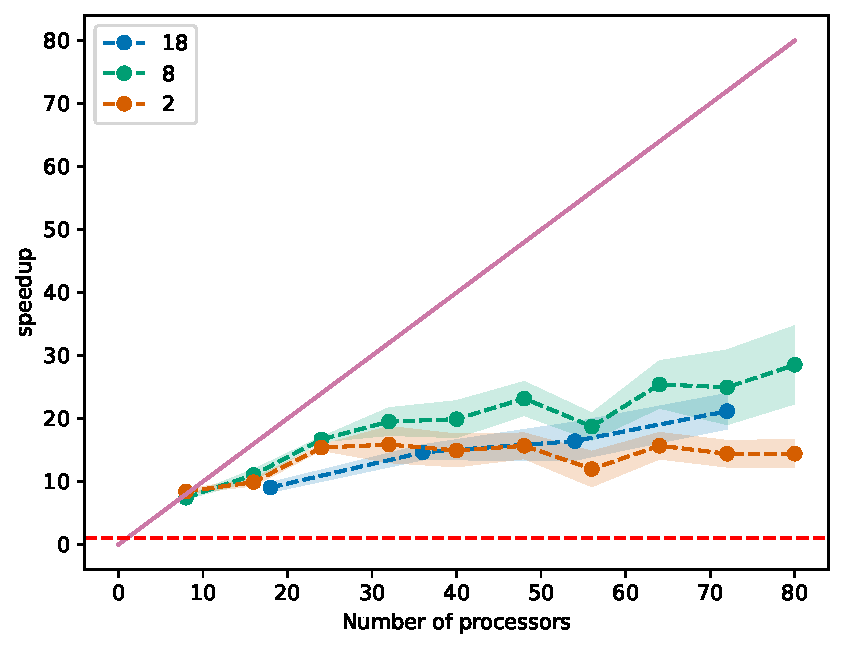
\includegraphics[width=0.7\textwidth]{plots_ph/si_ph_bench_nk_speedup.pdf}
    \caption{Scalability utilizing k-point parallelization for the Si benchmarking system with three sizes of processor pools, \emph{\QE compiled with \gls{oneapi} 2021.4, \texttt{nd 1}}}
    \label{fig:scaling_ph_nk_si}
\end{figure}
Interestingly, the result from the \texttt{PWscf} calculation on silicon from sec. \ref{sub:scf_scaling_k_point} is not reproduced here: the smallest pool size of 2 is not the one parallelizing best, but instead it is pool size 8.
Furthermore, for more than 50 processors, even the biggest pool size 18 shows better scaling than the pool size 2.
The general picture is similar to \texttt{PWscf} benchmark with k point parallelization on the \TaS benchmarking system in sec. \ref{sub:scf_scaling_k_point}, as there isn't an optimal pool size over the whole range of processors, instead some pool sizes seem to work best for some ranges.

\begin{figure}[htb!]
    \centering
    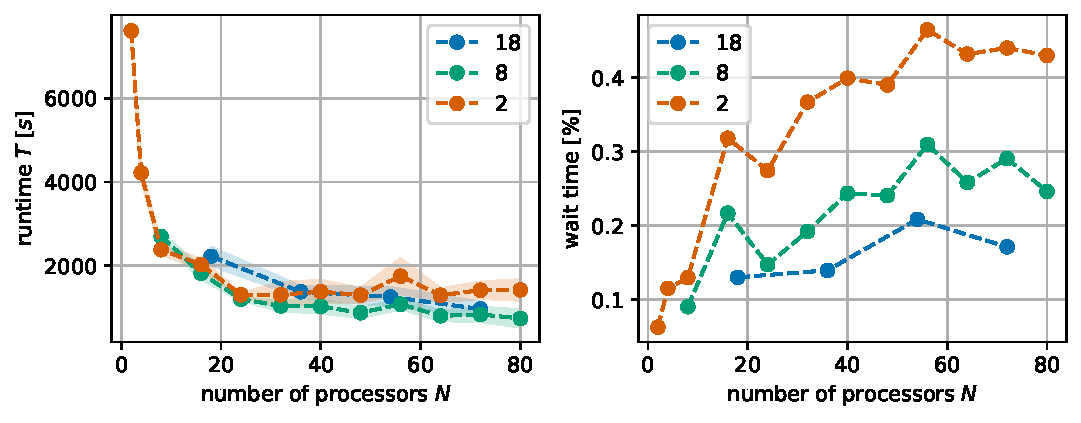
\includegraphics[width=\textwidth]{plots_ph/si_ph_bench_nk_absolute_wait.pdf}
    %\begin{subfigure}[b]{0.49\textwidth}
    %    \centering
    %    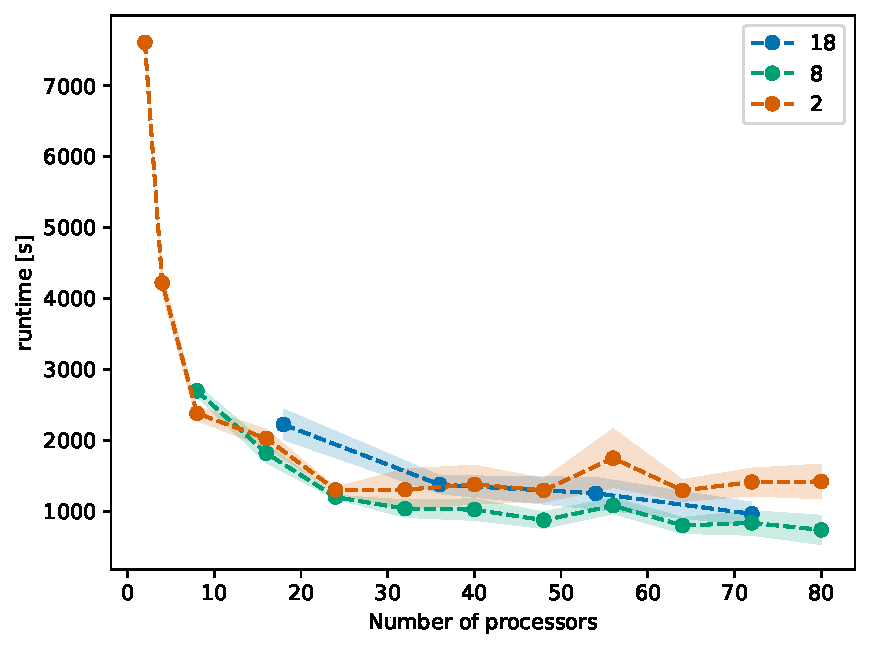
\includegraphics[width=\textwidth]{plots_ph/si_ph_bench_nk_absolute.pdf}
    %\end{subfigure}
    %\begin{subfigure}[b]{0.49\textwidth}
    %    \centering
    %    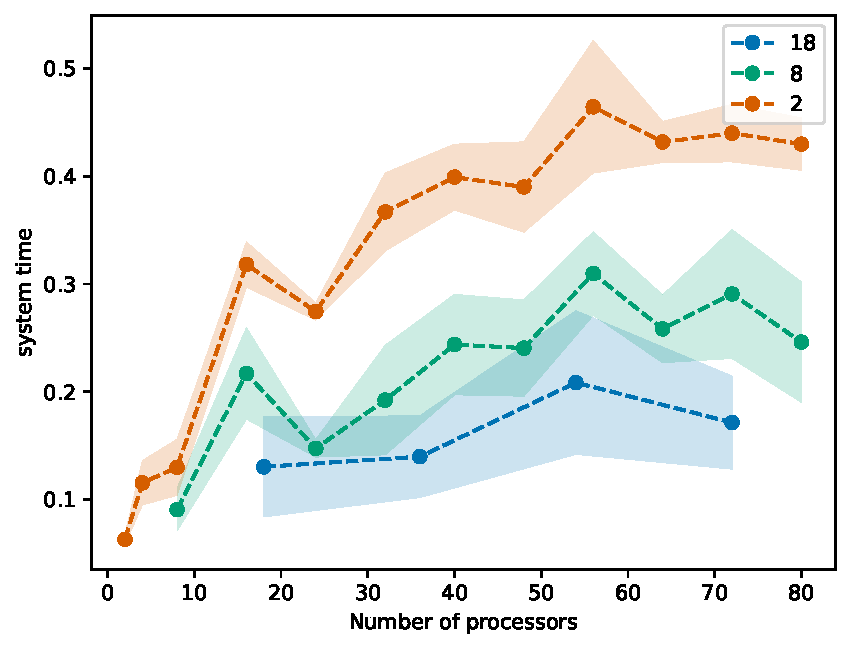
\includegraphics[width=\textwidth]{plots_ph/si_ph_bench_nk_wait.pdf}
    %\end{subfigure}
    \caption{Absolute runtime and wait time for the scalability test utilizing k-point parallelization for the Si benchmarking system with three sizes of processor pools, \emph{\QE compiled with \gls{oneapi} 2021.4, \texttt{nd 1}}}
    \label{fig:scaling_ph_nk_si_absolute_wait}
\end{figure}
One possible conclusion to draw from ch. \ref{ch:optimisation_scf} is that the longer runtime result in the calculation profiting more from parallelization and as such also from bigger pool sizes.
The phonon benchmark has a similar runtime to the \texttt{PWscf} benchmark on \TaS shown in sec. \ref{sub:scf_scaling_k_point}, so a similar scaling behavior should be expected.
Comparison in wait time reveals the differences in the quality of parallelization between the two systems, which results in the observed different scaling. 
Whereas the \texttt{PWscf} benchmark on \TaS had wait time not exceeding about \(\SI{8}{\percent}\) of the \gls{wall_time}, the wait time shown in fig. \ref{fig:scaling_ph_nk_si_absolute_wait} between \(\SI{10}{\percent}\) and \(\SI{50}{\percent}\).

A possible explanation for these differences between the two kinds of calculation can be found in how the time is actually spent during the calculation (which can be found in the \QE output files):
In the case of the phonon calculation on silicon, the time of one iteration is on the scale of seconds, whereas one iteration for the \texttt{PWscf} calculation on \TaS is about \(\SI{1}{\minute}\).
This means that the proportion of time spent on the distribution of data is bigger for the phonon calculation on silicon compared to the \texttt{PWscf} calculation on \TaS, which introduces wait times.

From the result of this benchmark, the parameters for the image parallelization in sec. \ref{sub:scaling_ph_images} can be set: the pool size will be fixed at 8.

\subsection{Linear algebra parallelization}

\begin{figure}[htb!]
    \centering
    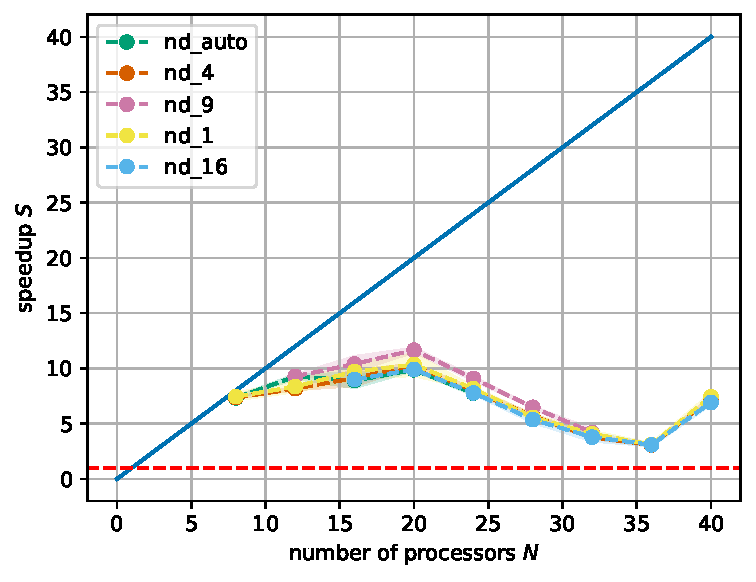
\includegraphics[width=0.75\textwidth]{plots_ph/si_ph_bench_nd_speedup.pdf}
    \caption{Scalability utilizing linear algebra parallelization for the Si benchmarking system, \emph{\QE compiled with \gls{oneapi} 2021.4, \texttt{nk 1}}}
    \label{fig:scaling_ph_nd_si}
\end{figure}
Fig. \ref{fig:scaling_ph_nd_si} shows that using linear algebra parallelization has so significant impact on the speedup.
This is again in contrast to the \texttt{PWscf} results from sec. \ref{sec:scf_scaling_qe_parallelization}, where using linear algebra slowed down the calculation.
This is again similar to the \texttt{PWscf} calculation on \TaS.

As such, linear algebra parallelization will not be used in the benchmarks for image parallelization.

\subsection{Image parallelization}\label{sub:scaling_ph_images}

When using image parallelization, \QE outputs a separate time report for every image, so one additional step is needed in the analysis:
While the total runtime of a calculation is determined by the longest running image, the variation of times between images is important to judge how well the work between images is distributed.
This is depicted in fig. \ref{fig:scaling_ph_ni_poolsize_8_si}.

\begin{figure}[htb!]
    \centering
    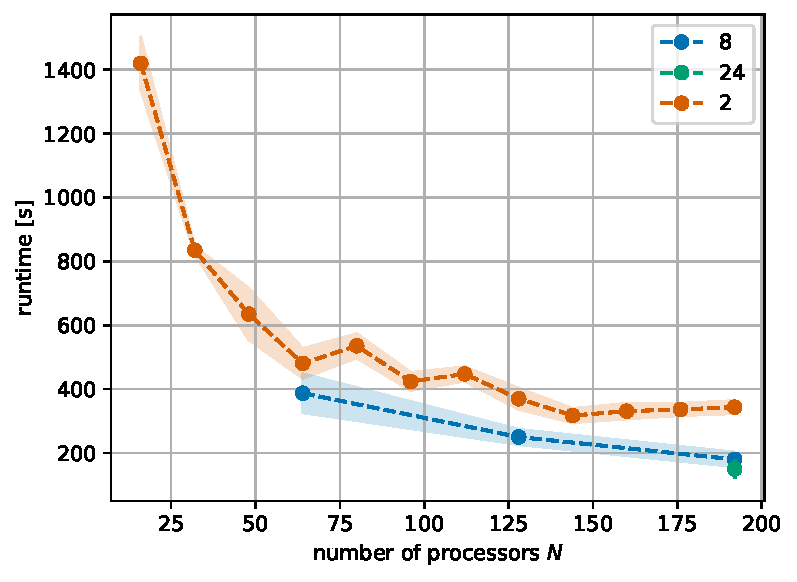
\includegraphics[width=0.75\textwidth]{plots_ph/si_ph_poolsize_8_images_distribution.pdf}
    \caption{Average runtime across images for the scalability test utilizing image and k point parallelization on the Si benchmarking system with three values of \emph{\texttt{ni}}, \emph{\QE compiled with \gls{oneapi} 2021.4, \texttt{nk, ni} chosen such that poolsize = 8, \texttt{nd 1}}}
    \label{fig:scaling_ph_ni_poolsize_8_si_distribution}
\end{figure}
As the times between images are quite constant, good load balancing between images can be assumed for the silicon benchmarking system.


With the maximum time across images, speedup is then calculated, shown in fig. \ref{fig:scaling_ph_ni_poolsize_8_si}.

\begin{figure}[htb!]
    \centering
    %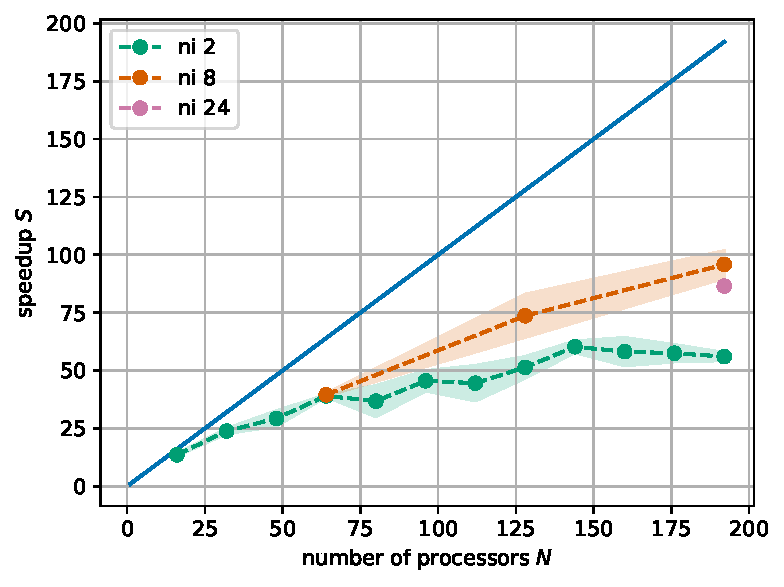
\includegraphics[width=0.75\textwidth]{plots_ph/si_ph_poolsize_8_bench_ni_speedup.pdf}
    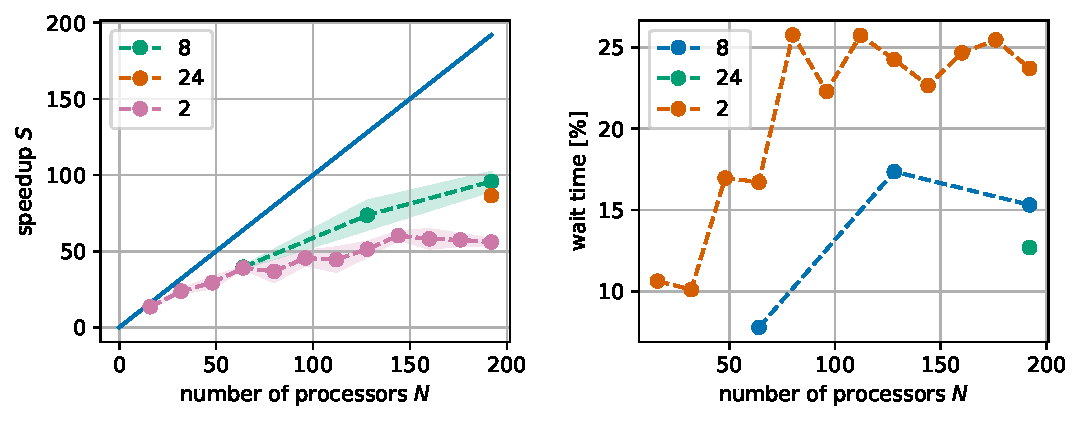
\includegraphics[width=\textwidth]{plots_ph/si_ph_poolsize_8_bench_nk_speedup_wait.pdf}
    \caption{Speedup and wait time calculated from the longest running image for the scalability test utilizing image and k point parallelization on the Si benchmarking system with three values of \emph{\texttt{ni}}, \emph{\QE compiled with \gls{oneapi} 2021.4, \texttt{nk, ni} chosen such that poolsize = 8, \texttt{nd 1}}}
    \label{fig:scaling_ph_ni_poolsize_8_si}
\end{figure}
The speedup shows that using image parallelization helps the phonon calculations scale over more processors than just using k point parallelization.
Even just using 2 images almost doubles the maximal achieved speedup in fig. \ref{fig:scaling_ph_nk_si}.
This behavior doesn't extend across the whole range of processors, but using more images can partially elevate this problem.

The wait time (also calculated from the longest running image) shown in fig. \ref{fig:scaling_ph_nk_si_absolute_wait} is particularly good for every first data point, so in cases where only image parallelization without additional k point parallelization is applied.
As an example, for 64 processors, 8 images is \(\nicefrac{N_P}{N_i} = 8\), so the pool size is already 8 as required and the parameter \texttt{nk} is chosen to be 1.
So at least for the silicon system it seems to be advisable to choose the parameter \texttt{ni} as large as possible, so that \texttt{nk} can be chosen as small as possible while keeping a pool size of 8.

\section{Phonon calculations on \TaS}\label{sec:phonon_tas2}

The results from the last section can be used to estimate good parallelization parameters for a phonon calculation at the \(\mathrm{\Gamma}\) point for \TaS in the charge density wave phase.
The calculations were run on 180 processors, once with the previous established optimal pool size of 36 and once with a pool size of 18 for comparison.
The relevant benchmark values for this calculation are listed in tab. \ref{tab:tas2_cdw_phonon_times}.

\begin{table}[ht!]
    \caption{Benchmark values for phonon calculations of \TaS in the charge density wave phase, run on 180 processors}
    \begin{tabular}{@{}lll@{}}
    \toprule
                 & runtime            & wait time \\ \midrule
    pool size 18 & \SI{3044}{\minute} & \SI{16}{\percent}         \\
    pool size 36 & \SI{2020}{\minute} & \SI{7.4}{\percent}
    \end{tabular}
    \label{tab:tas2_cdw_phonon_times}
\end{table}
In this calculation the need for a good choice of parallelization parameters becomes especially clear:
on the on the same number of processors, with the only difference in the choice of the parameter \texttt{nk}, the two calculations have a difference of \(\SI{17}{\hour}\).

\section{Conclusion: Parameters for optimal scaling}

The benchmarks on \QE's \texttt{PHonon} module showed that calculation on the silicon system profited more from bigger k point pools than \texttt{PWscf} calculations.
Linear algebra parallelization was shown to have no impact on calculations.

Image parallelization in combination with k point parallelization lead to very good scaling across a wide range of processors.
Best results were found when the processors were only split up by image parallelization.

Phonon calculations on \TaS in the charge density wave phase were then carried out, with the best time reached for a pool size of 36.

\end{document}